
\begin{figure}
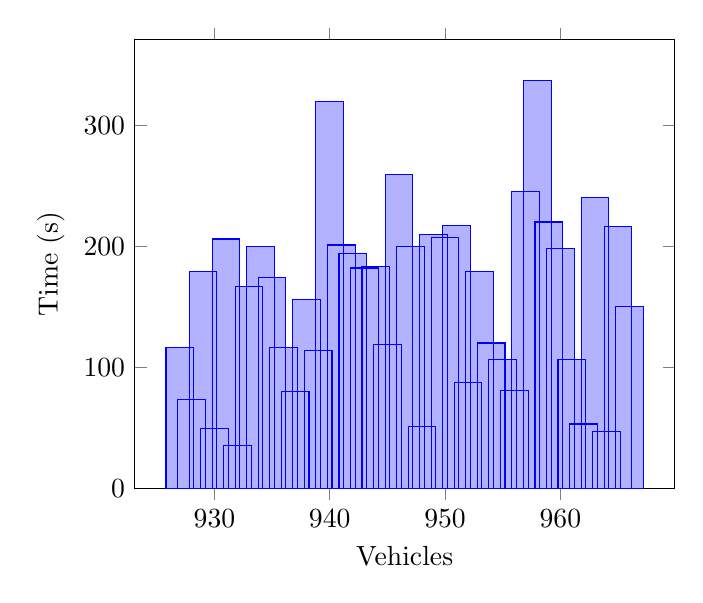
\begin{tikzpicture}
\begin{axis}[
legend style={anchor=west},
xlabel=Vehicles,
ylabel=Time (s),
ymin=0,
ybar,
]
\addplot coordinates {
(947, 200)
(942, 194)
(957, 245)
(964, 47)
(955, 106)
(929, 179)
(945, 119)
(966, 150)
(953, 179)
(956, 81)
(931, 206)
(930, 49)
(935, 174)
(941, 201)
(963, 240)
(958, 337)
(934, 200)
(937, 80)
(954, 120)
(936, 116)
(927, 116)
(961, 106)
(944, 183)
(950, 207)
(940, 320)
(951, 217)
(949, 210)
(962, 53)
(932, 35)
(952, 87)
(928, 73)
(948, 51)
(933, 167)
(946, 259)
(965, 216)
(943, 182)
(960, 198)
(959, 220)
(938, 156)
(939, 114)
};

\end{axis}
\end{tikzpicture}
\label{tik:time:100:13}
\caption{100 percent diving with GSC on route $13$}
\end{figure}
